Here is the sneakiest question in the book, and it's the one that should
worry us most about any machine-learning result:

\begin{quote}
\textbf{When the model does well, is it doing the computation --- or
just recognizing the words?}
\end{quote}

A model that maps the phrase ``the sum of a and b'' to \texttt{a\ +\ b}
might not be doing arithmetic at all. It might be doing something much
dumber: associating the \emph{exact phrasing} it saw in training with
the code that followed it. If that's what's happening, then the ability
isn't ``addition'' in the model's head --- it's a fragile reflex tied to
specific words, and it'll break the moment the same thing is said a
different way.

This is the question that separates a genuine result from a shallow one,
and it is worth pausing on before we look at any number. Consider what a
``yes, it just recognized the words'' answer would mean. It would mean
that every high score the model achieved --- every impressive
in-distribution number --- was not evidence of learning at all. It was
evidence of association. The model did not learn to add; it learned that
a particular sentence means \texttt{return\ a\ +\ b}. That is a
completely different claim, and it is the one we need to test.

\section{The design: change what shouldn't
matter}\label{the-design-change-what-shouldnt-matter}

To find out, we run the \textbf{surface-generalization} test. The logic
is simple and elegant: if we change something that \emph{shouldn't}
change the computation --- the variable names, or the wording --- and
the model fails, then it never really learned the computation. It
learned the phrasing.

The key is choosing \emph{what} to change. We want to change only the
\emph{surface} --- the outer layer of the sentence --- and leave the
underlying computation completely untouched. Swapping \texttt{a} and
\texttt{b} for \texttt{left} and \texttt{right} does not change what
``add these two numbers'' means. Rewording ``their sum'' as ``the
total'' does not change the operation. If the model truly understood
addition, neither change would matter. If it merely memorized a
sentence, either change would break it. That asymmetry is exactly what
we measure.

We designed a set of controlled surface changes, each one
\emph{supposedly harmless} to the underlying task, and tested the model
on each. This is the crux of the book's approach to generalization: we
do not just ask ``does it work?'' We ask ``does it survive the changes
that a genuinely-general system should shrug off?''

\section{The setup}\label{the-setup}

We trained the model on arithmetic primitives, but only with
\textbf{letter names} (\texttt{a}, \texttt{b}) and only a \textbf{subset
of the wording} used to describe each operation. Then we re-asked the
\emph{identical} task three different ways and watched whether the
model's ability survived.

\section{The result}\label{the-result}

\begin{longtable}[]{@{}llll@{}}
\toprule\noalign{}
Test & \textbf{MODEL} & TEMPLATE & RETRIEVAL \\
\midrule\noalign{}
\endhead
\bottomrule\noalign{}
\endlastfoot
Same as training & \textbf{0.900} & 0.800 & 1.000 \\
Same computation, \texttt{a,b} → \texttt{left,right} & \textbf{0.350} &
0.800 & 0.683 \\
\textbf{Same computation, reworded} & \textbf{0.000} & 0.875 & 0.125 \\
\end{longtable}

Look at what happens when we touch only the \emph{surface}, not the
math.

\begin{itemize}
\item
  \textbf{New variable names.} The model was trained on \texttt{a} and
  \texttt{b}. We ask the same question with \texttt{left} and
  \texttt{right} --- the \emph{identical} operation. Performance
  collapses from \textbf{0.900 to 0.350}.
\item
  \textbf{Reworded instruction.} We say the exact same problem using a
  phrasing the model never saw during training. Performance drops to
  \textbf{0.000}.
\end{itemize}

So the model that scored 0.900 on the familiar phrasing falls to 0.350
when the variable names change, and to 0.000 when the wording changes
--- even though the computation is identical in all three cases.

\section{The damning comparison}\label{the-damning-comparison}

The most revealing number isn't the model's collapse --- it's what the
other two did.
\pandocbounded{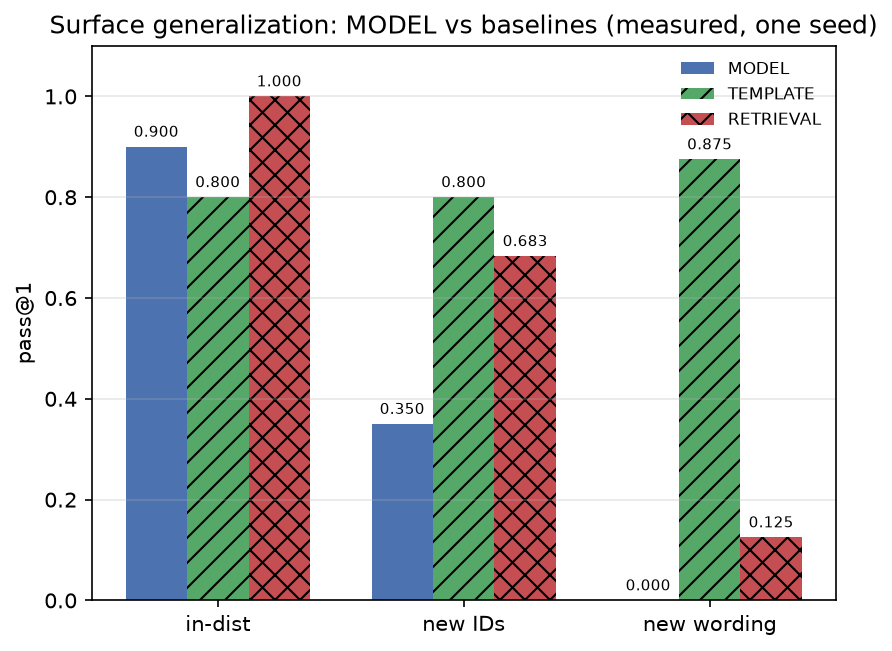
\includegraphics[keepaspectratio,alt={Surface generalization},width=\maxwidth{\textwidth},keepaspectratio]{figures/fig_surface.png}}

When we change the \emph{words}, the \textbf{template baseline gets
\emph{better}, not worse} (0.875, up from 0.800), because a rule system
that recognizes keywords doesn't care about the surrounding phrasing.
The \textbf{retrieval baseline} also holds up (0.683). Only the
\textbf{learned model} falls apart --- because the model learned the
\emph{specific sentences}, not the \emph{idea}.

So the model's 0.900 in-distribution score was largely \textbf{phrasing
memorization}. It had learned ``this exact kind of sentence maps to that
program.'' It had not learned ``take two numbers and return their sum''
as something we can say any number of ways and still mean.

This inversion --- where the neural model is \emph{worse} than a dumb
rule system under surface change --- is the most informative signal in
the experiment. It is not a competitive defeat; it is a diagnostic
revelation. The dumb template system is indifferent to exact wording
because it never learned to associate wording with meaning in the first
place; it just recognizes keywords. The neural model, by contrast, bound
the operation to the \emph{particular words}, so when the words change,
the binding snaps. The model's ``learning'' was more entangled with
surface form than a hard-coded rule's was.

\section{The brewing experience}\label{the-brewing-experience}

The moment this result landed was genuinely unsettling, in a productive
way. We had just celebrated the 0.900 in-distribution score --- the
model, we thought, could ``add.'' Then we reworded the same problem and
the floor fell out. The 0.900 had been real, and it had been
\emph{narrow}. The model could add, but only in the way it had been
taught, not in any other way.

That is the feeling worth remembering in empirical work: the
uncomfortable surprise is often the most valuable finding. It would have
been easy to stop at ``the model scores 0.900, success.'' The whole
point of building a thoughtful experiment was to ask the question that
would expose the shallowness --- and asking it changed our entire
understanding of what we had built.

\section{The shortcut audit}\label{the-shortcut-audit}

\begin{enumerate}
\def\labelenumi{\arabic{enumi}.}
\item
  \textbf{Suspected cheat: phrasing memorization.} \textbf{Why it fits:}
  the model tied training phrasings to code. \textbf{Control:} held one
  whole phrasing style out of training, tested on it. \textbf{Result:}
  0.000. \textbf{Ruled out:} that the model is grounded in the
  computation. \textbf{Still open:} is it the wording pattern or the new
  vocabulary? Need a surface-control to separate them.
\item
  \textbf{Suspected cheat: name memorization.} \textbf{Why it fits:}
  trained on \texttt{a,b}, maybe it hardwired those labels.
  \textbf{Control:} retest on \texttt{left,right}. \textbf{Result:}
  0.350 --- a big but partial drop. \textbf{Ruled out:} pure
  name-memorization (it still fails partly, but names aren't the whole
  story).
\end{enumerate}

\section{The honest takeaway}\label{the-honest-takeaway}

A model that scores 0.900 on familiar phrasings and 0.000 on a rewording
of the same problem has not generalized to the \emph{problem}. It
generalized to the \emph{phrasing}. That's the difference between ``the
model works'' and ``the model works when I say it the way I said it in
training'' --- and it's the most important lesson of the generalization
chapters.

The sharpest way to state it: the model did not learn \emph{addition}.
It learned the \emph{word ``sum''}. When that word appears in the
sentence it was trained on, the model produces \texttt{a\ +\ b}. When
the same meaning arrives in different words, the model has no idea what
to do. And that is the difference between a system that understands and
one that merely recites.
